%! Author = lili
%! Date = 4/22/26

\section{Auftrennung von doppelsträngiger DNA}
\frage{dnatrennung}

\begin{figure}[H]
    % TODO Schmelzkurve 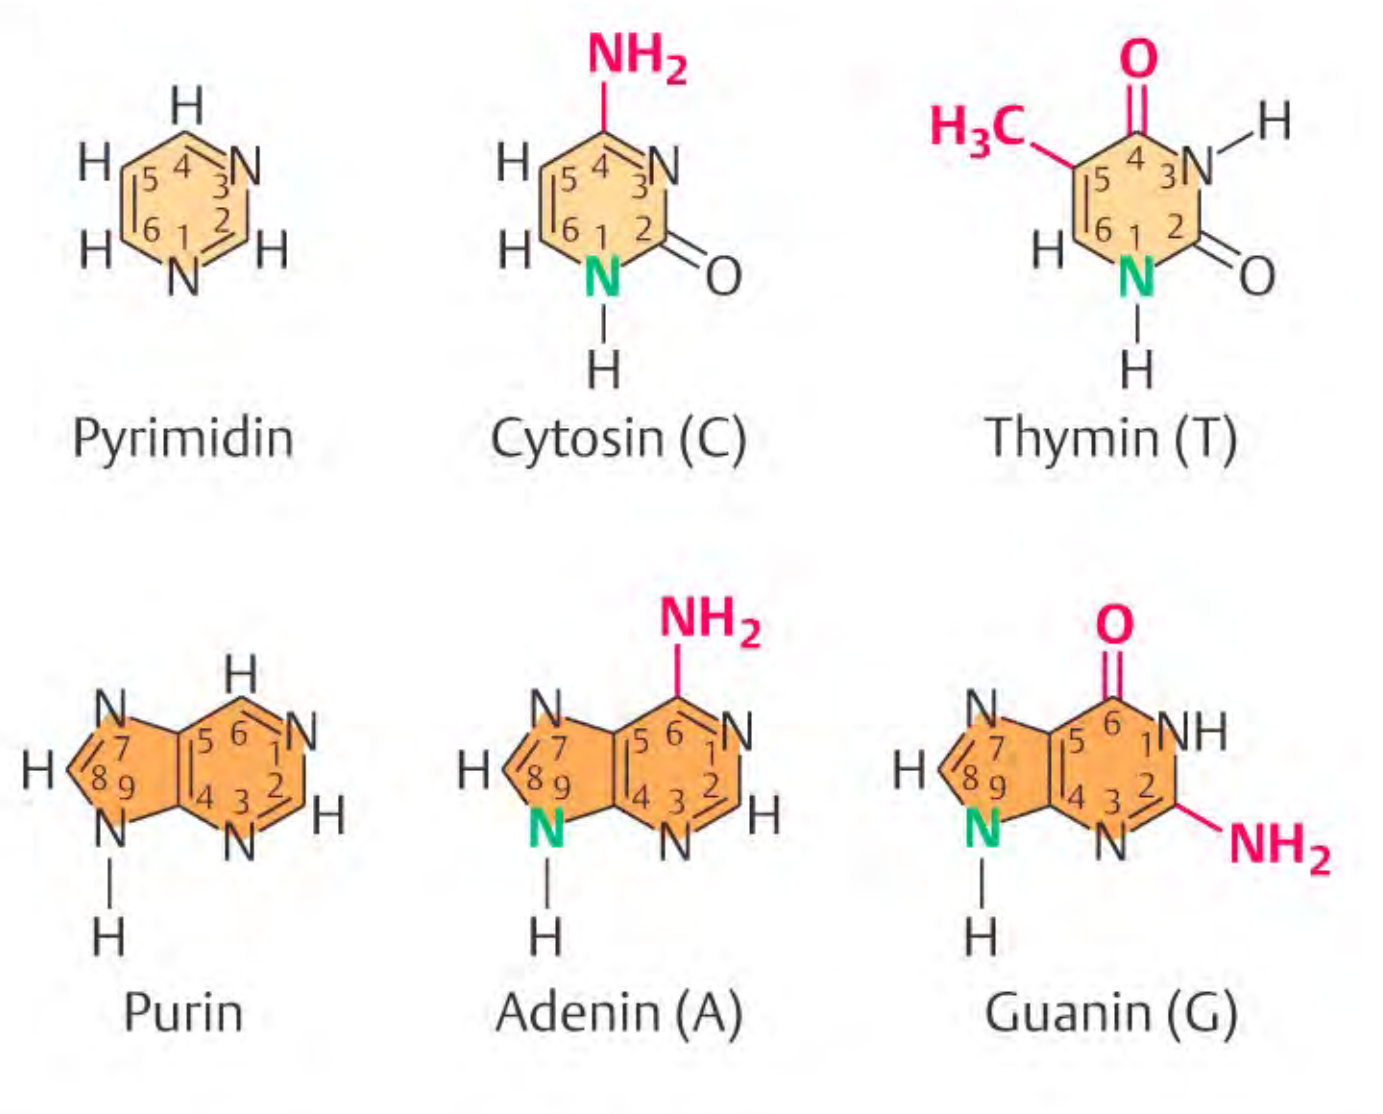
\includegraphics[width=\textwidth]{bilder/basen}
    \caption{Die Schmelzkurve der DNA}
\end{figure}

\defin{cot-analyse}

\section{Das Genom}

\defin{Genom}

\defin{Nukleom}

\defin{Plastom}

\defin{Chondrom}

\section{DNA-Replikation}

\defin{konRep}
\defin{disRep}
\defin{semiRep}

\defin{biRep}

\subsection{Start der Replikation}
\defin{oric}

\begin{figure}[H]
    % TODO F26 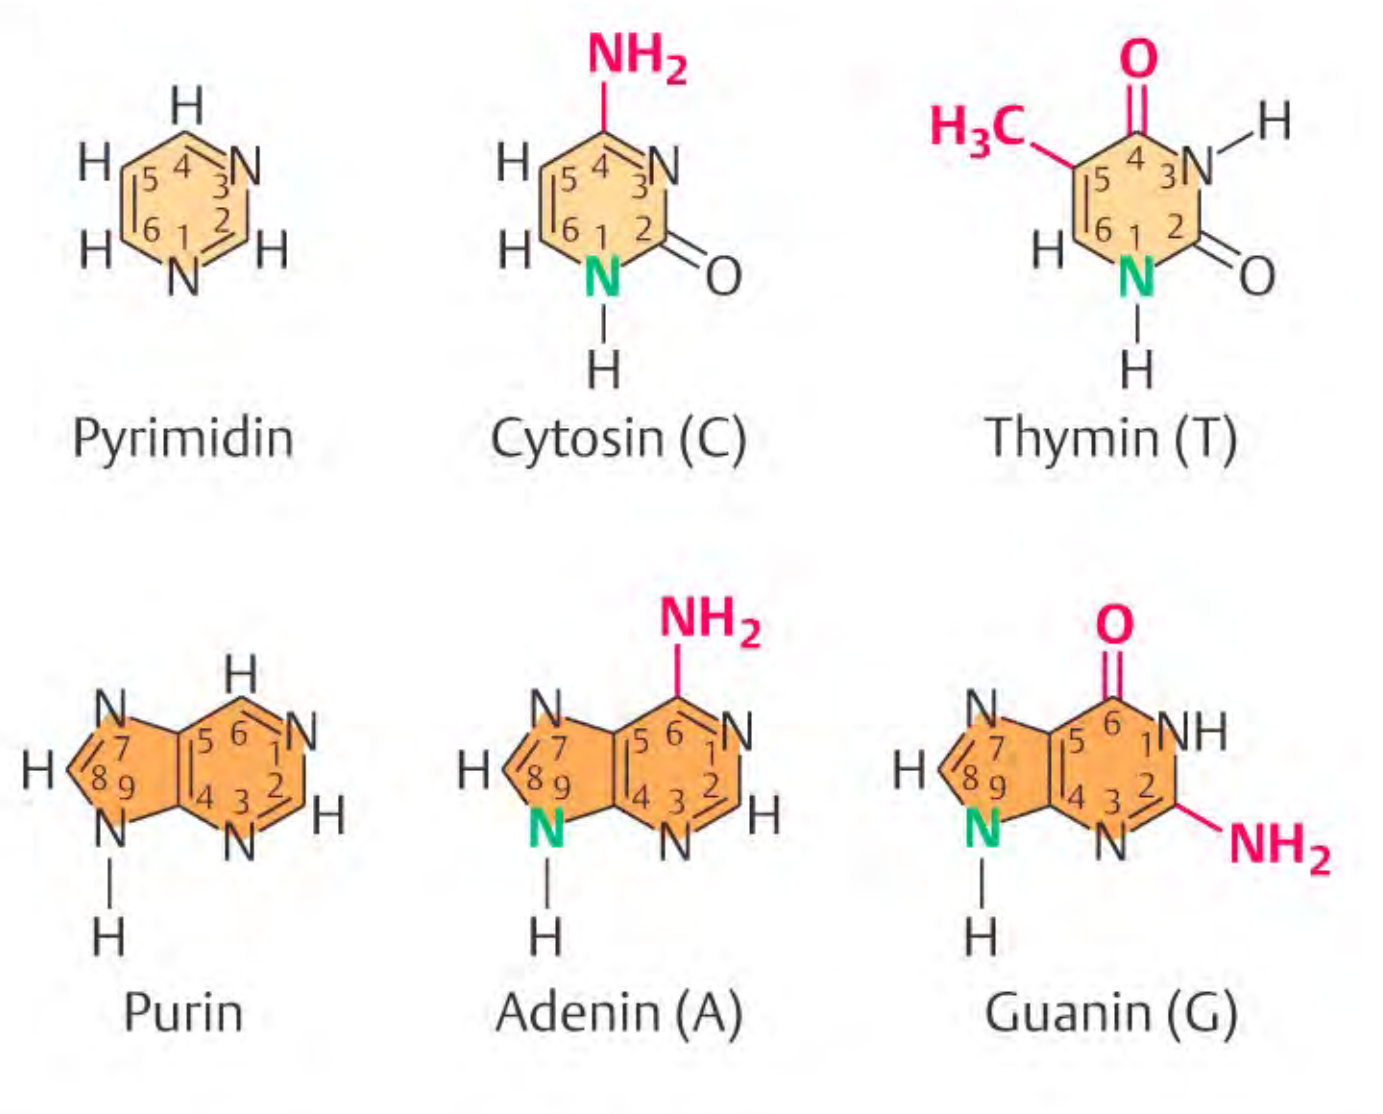
\includegraphics[width=\textwidth]{bilder/basen}
    \caption{Start der Replikation am oriC.}
\end{figure}

\subsection{DNA-abhängige DNA-Polymerase}
Alle DNA-Polymerasen benötigen einen Primer...
% TODO F27

\subsection{Die Replikationsgabel}
% TODO F28, 34

\subsection{Primase und DNA-Polymerase III}
% TODO F32-33, 35

\subsection{Die DNA-Polymerase I}

\begin{bsp}
    \textbf{Die DNA-Polymerase I von E. coli}
    % TODO 38 - 43
\end{bsp}

\subsection{Weiterer Verlauf der Replikation}

% TODO 60-63

\subsection{Abschluss der Replikation}

\section{DNA-Superhelikalität}

% TODO F 49 - 55, 60

\begin{bsp}
    \textbf{Replikation des Escherichia coli-Chromosoms}
\end{bsp}

\section{DNA Topoisomerasen}

% TODO F 56-58
